\documentclass[addpoints]{exam}

\usepackage{graphicx}
\usepackage{hyperref}
\usepackage{subcaption}

% Header and footer.
\pagestyle{headandfoot}
\runningheadrule
\runningfootrule
\runningheader{CS 201 Data Structures II}{HW 3: Information Retrieval}{Spring 2021}
\runningfooter{}{Page \thepage\ of \numpages}{}
\firstpageheader{}{}{}

\qformat{{\large\bf \thequestion. \thequestiontitle}\hfill}
\boxedpoints

\noprintanswers

\graphicspath{{images/}}

\title{Homework 3: Information Retrieval\\Moogle -- My Awesome Google}
\author{CS 201 Data Structures II\\Habib University\\Spring 2021}
\date{Due: 2359h on Sunday, 21 Mar}

\begin{document}
\maketitle

\begin{figure}[h]
  \centering
  
\includegraphics[width=.9\textwidth]{guardian}
  \caption{\href{https://www.theguardian.com/world/coronavirus-outbreak}{Coronavirus Outbreak $|$ The Guardian}, accessed Sunday, 22 March, 2020.}
  \label{fig:guardian}
\end{figure}

\begin{figure}
  \centering
  \begin{subfigure}{.7\textwidth}
    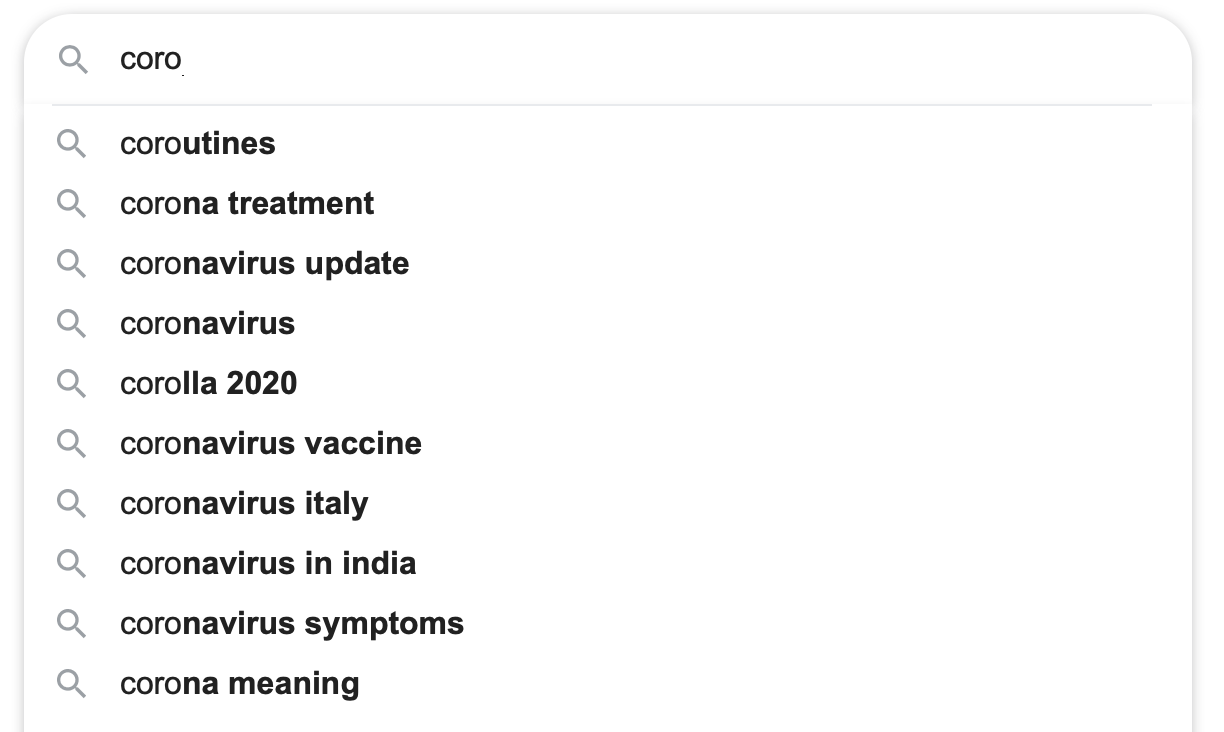
\includegraphics[width=\textwidth]{autocomplete}
    \caption{An example of auto-complete suggestions from \url{https://www.goole.com}.}
    \label{fig:autocomplete}
  \end{subfigure}
  \begin{subfigure}{.2\textwidth}
    
\includegraphics[width=\textwidth]{moogle}
    \caption{Not this \href{https://finalfantasy.fandom.com/wiki/Final_Fantasy_Wiki}{Moogle}!}
    \label{fig:moogle}
  \end{subfigure}
\end{figure}

In this assignment you will build Moogle (My Google), a system to perform information retrieval tasks on a corpus. Specifically, Moogle will perform 2 tasks.
\begin{enumerate}
\item Given a query, find completion matches for it from the corpus. For example, see Figure \ref{fig:autocomplete}.
\item Given a query, retrieve a list of documents from the corpus ranked according to their relevance to the query.
\end{enumerate}

The first task is supported by building a trie with all the words in the corpus. The second is supported by an inverted index built from all the documents from the corpus. You will write the necessary functionality without building the interface.

The corpus consists of 3028 news articles published between 1 January, 2020 and 21 March, 2020 matching the keyword, ``coronavirus'', and retrieved through \href{https://open-platform.theguardian.com}{the API} of \href{https://www.theguardian.com/}{The Guardian}. You may obtain it from \href{https://drive.google.com/file/d/1yCDm2d3Jj6Z5XcG_ut7mKB-gnWpjDc_S/view?usp=sharing}{here}.

\section{Tokenization}

An important operation in this context is \href{https://nlp.stanford.edu/IR-book/html/htmledition/tokenization-1.html}{tokenization} which breaks a long string into smaller strings or \textit{tokens} which are more appropriate for the application. There is no \textit{correct} or \textit{standard} tokenization, rather different applications require the string to be tokenized differently. This operation features repeatedly in our implementation.

\section{Implementation}

The accompanying implementation provides the following classes and supporting helpers.

\paragraph{\texttt{Corpus}} It encapsulates a \texttt{Trie} and an \texttt{Index} and supports completion and search queries as described above by delegating to the appropriate member structure. A \texttt{Corpus} instance is initiated with the path to a directory containing the documents to be processed. The documents must be in \texttt{.txt} format.

\paragraph{\texttt{Document}} A representation of a document in the corpus. It processes a \texttt{.txt} file and offers it in a manner suitable for the other structures. It uses the helper, \texttt{document\_tokenize}, to tokenize the content of the document. You may leave the helper unchanged initially. Each \texttt{Document} instance also stores an ID in order to uniquely identify the document from which it derives.

\paragraph{\texttt{Location}} Represents the location of a word in the corpus. A word may appear in multiple locations in the same document and in multiple documents. The \texttt{Location} class stores document ID and the start and stop indexes (as per python slicing convention). Many of the functions in the provided implementation that deal with words also expect an accompanying list of \texttt{Location} objects.

\paragraph{\texttt{TrieNode}} A node in the trie. It simply contains a dictionary (hash table) that maps letters in the alphabet to children. Note that the node does not store a label.

\paragraph{\texttt{Trie}} A \texttt{Trie} contains its root node and 2 methods. It uses \texttt{\^} as the string terminating character. Labels are stored not in the nodes but in the edges, or more specifically as the keys in the \texttt{children} dictionary at each node. The node corresponding to the last letter of a word has an entry in its dictionary with the terminator as key and the list of \textit{Location}s as value.
\begin{itemize}
\item The \texttt{add\_doc} method adds a document to the trie. Each word from the document is first preprocessed using a helper, \texttt{trie\_preprocess}, which you can initially leave unchanged, and the result is then added to the trie using another helper, \texttt{add\_word}, which you have to implement.
\item The \texttt{complete} method returns matches from the trie to given prefixes which are passed in as a single space separated string. It uses the helper, \texttt{prefix\_tokenize}, to tokenize the received string into individual prefixes. You can initially leave this helper unchanged. The actual matching uses another helper, \texttt{match}, which you have to implement.
\end{itemize}

\paragraph{\texttt{Index}} The inverted index supports TF-IDF matching of a query to the stored documents.
\begin{itemize}
\item The \texttt{add\_doc} method adds a \texttt{Document} to the index and has to be implemented by you. Before addition to the index, each word from the document should be pre-processed by the helper, \texttt{index\_preprocess}, which you can initially leave unchanged.
\item The \texttt{query} method takes a single space separated query string to return a ranked list of document IDs. It should be implemented by you. The query string should first be tokenized using the helper, \texttt{query\_tokenize}, which you may initially leave unchanged.
\end{itemize}

\section{Tasks}

You have to implement the following functions.
\begin{itemize}
\item the \texttt{add\_word} helper to \texttt{Trie}
\item the \texttt{match} helper to \texttt{Trie}
\item the \texttt{\_\_init\_\_} method of \texttt{Index}
\item the \texttt{add\_doc} method of \texttt{Index}
\item the \texttt{query} method of \texttt{Index}
\end{itemize}

\noindent For better results (see Section \ref{sec:refine}), you may also have to modify the following helpers.
\begin{itemize}
\item \texttt{document\_tokenize}
\item \texttt{trie\_preprocess}
\item \texttt{prefix\_tokenize}
\item \texttt{index\_preprocess}
\item \texttt{query\_tokenize}
\end{itemize}

There should not be a need to modify any of the other code.

\section{Fine Tuning}
\label{sec:refine}

Congratulations, you have implemented your (very first) search engine! Be proud and play around with Moogle. Go over some of the documents, perform some searches, verify them, try out some completion results, and so on.

In so doing, you will begin to realize some quirks. You may come across strange characters (these are due to unhandled Unicode characters in the original documents). Stop words will pop up. Punctuation is not correctly handled. Some of the original documents are also strange--they contain little to no content, more strange characters. All of this is common in information retrieval.

In this section, you will refine your search engine to make it even more awesome!

Make a new branch in your repository called \texttt{awesome} to include your refinements. The \texttt{master} branch will contain code to meet basic functionality and pass Travis tests. Add a section called \textit{Refinements} at the end of the \texttt{README} in the \texttt{awesome} branch where you will list all the refinements that you incorporate. There are no specific instructions for these refinements and you are free to implement what you like. Some refinements are a matter of personal taste, so for each refinement include a line or two to explain why you think that refinement improves your search engine.

\subsection{Document Cleaning (Garbage In Garbage Out)}

Your results are only as good as your input and the quirks mentioned above are typical problems faced in Information Retrieval. That is why significant effort is spent on \textit{document cleaning}, i.e. reading or processing the documents to a form appropriate for further processing. In our setup, this will be handled by the \texttt{document\_tokenize} helper. Make appropriate refinements to \texttt{document\_tokenize} so that documents are better handled. Make sure to include each incorporated refinement in the \texttt{README}. 

\paragraph{Stop Words and Punctuation} How should your system handle stop words and punctuation? The usual practice is to leave them out. You may implement this functionality in \texttt{document\_tokenize} or in the individual tokenization functions of \texttt{Trie} or \texttt{Index}.

\paragraph{Stemming} Should documents containing the word ``doctors'' match a query for ``doctor''? How about ``isolate'' and ``isolation''? Should ``driving'' appear as a completion for ``drive''? The usual answer is ``yes''. These pairs of words are said to have the same \textit{stem} and reducing a word to its stem is called \textit{stemming}. You can best decide at what level to perform stemming--at the document level, for the trie, or for the index--and modify the corresponding functions. Make sure to justify your choice in your \textit{Refinements} section in the \texttt{README}.

\paragraph{Others} How about case sensitivity, words with apostrophe, e.g. ``don't'', how to handle quotation marks, and initials, e.g. ``George W. Bush''? Feel free to incorporate related refinements and explain them in your \texttt{README}.

\paragraph{Even More} The next level of search is ``semantic search'' where matching takes into account not only keywords but also their \textit{meaning}, e.g. the system can distinguish between ``who'' and ``WHO'', between ``pen'', the writing instrument, and ``pen'', the holding area for animals. Such pairs of words are called \textit{homonyms} and are one of the many exciting challenges that Information Retrieval deals with. There is no expectation from you to address them in this assignment.

\paragraph{\texttt{nltk}} As we see above, Information Retrieval has strong overlaps with Natural Language Processing (NLP). As such you may find the \href{https://www.nltk.org}{\textit{Natural Language Toolkit (ntlk)}} in python to be especially useful as you refine Moogle.


\section*{Credits}

This homework and related files are courtesy of \href{http://qasimpasta.info}{Muhammad Qasim Pasta}.

\end{document}

%%% Local Variables:
%%% mode: latex
%%% TeX-master: t
%%% End:
